\subsection{Threading}
For at simplificere opstart af tråde er klassen ThreadStarter blevet implementeret. Dens statiske metode, Start() tager imod objekter, som implementerer interfacet IThreadRunner. Disse objekter får kald RunThread(), hvori tråden eksekveres. ThreadStarter.Start() returnerer et .NET Thread objekt, som allerede er startet. Gennem Thread objektet kan tråden manipuleres (Stop, Join mv.).

\begin{figure}[H]
    \centering
    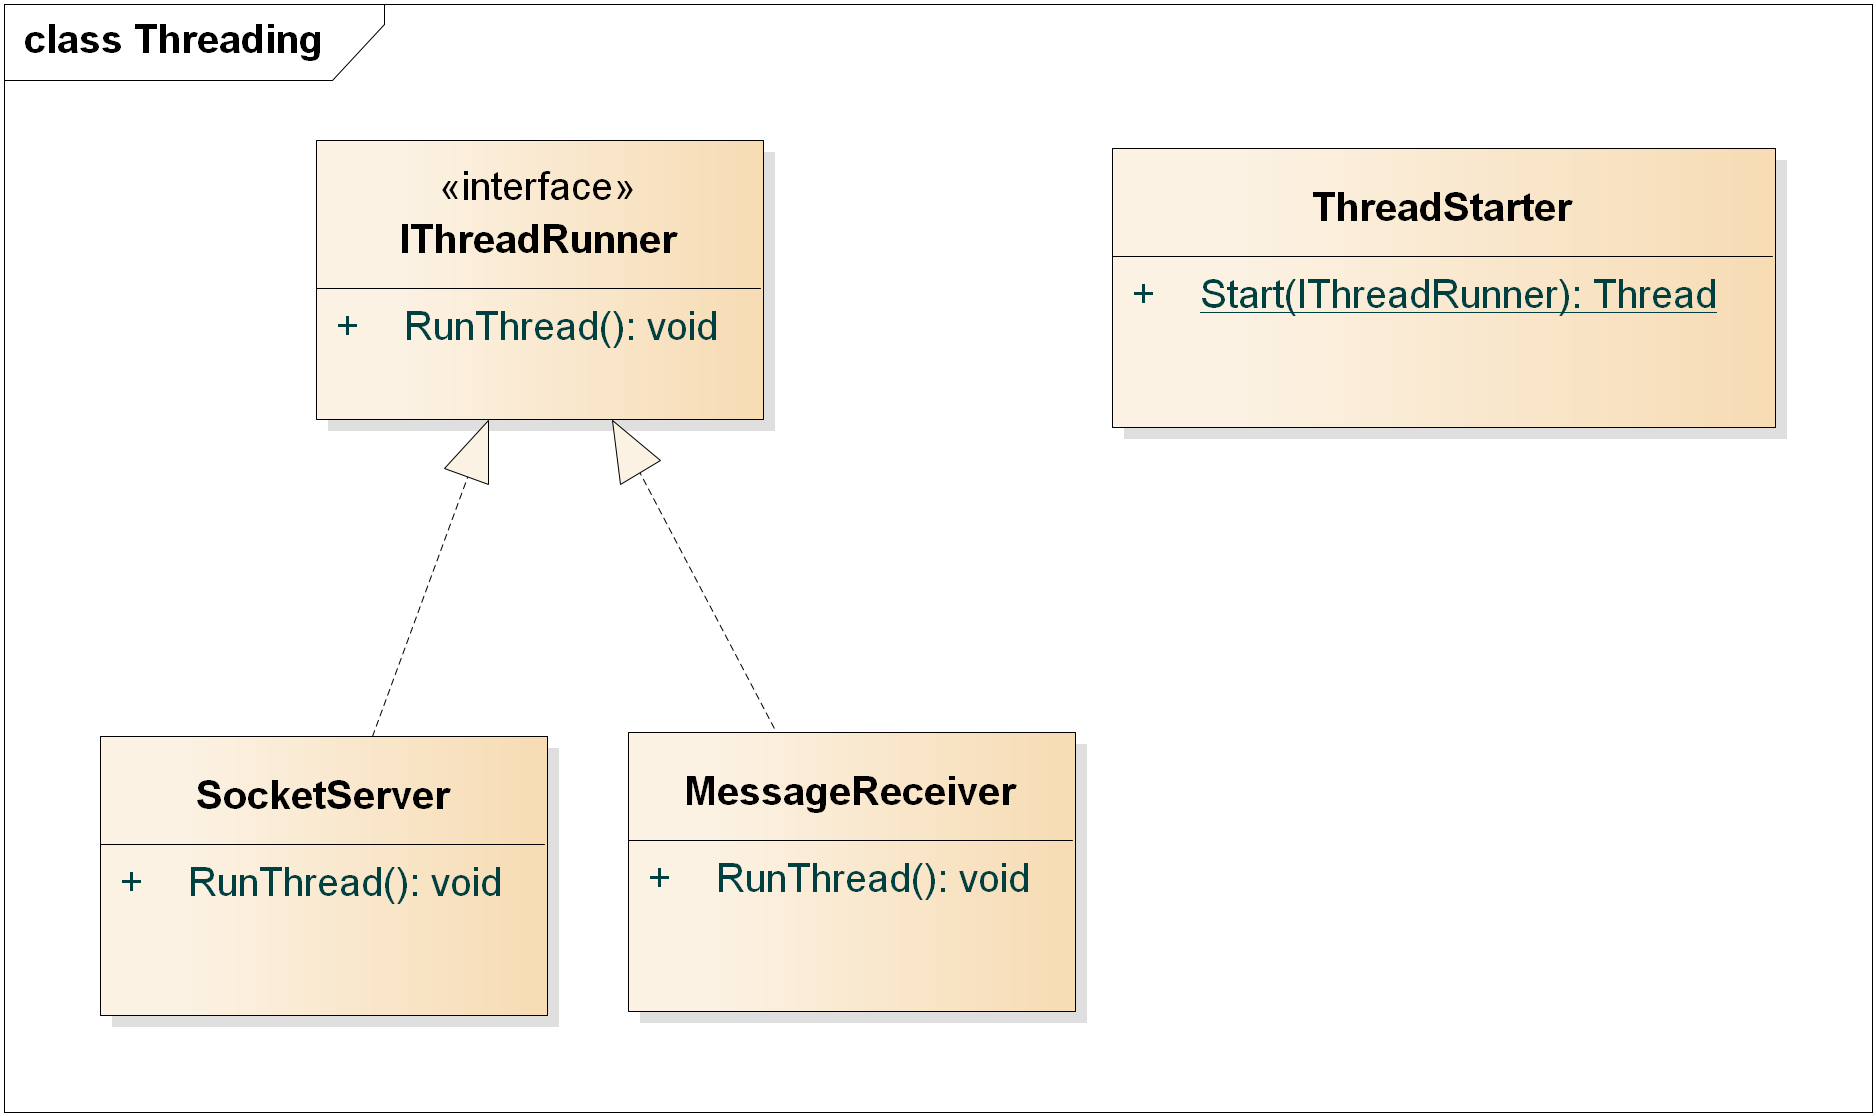
\includegraphics[width=1\textwidth]{Systemdesign/CentralServer/Images/Threading.png}
    \caption{UML-diagram for Threading pakken}
    \label{fig:CSThreading}
\end{figure}

I CentralServer implementerer følgende klasser IThreadRunner interfacet: SocketServer og MessageReceiver.